% Options for packages loaded elsewhere
\PassOptionsToPackage{unicode}{hyperref}
\PassOptionsToPackage{hyphens}{url}
%
\documentclass[
]{book}
\title{Day 4: One-Way and Two-Way ANOVA using R}
\author{Rey R. Cuenca\footnote{MSU-Iligan Institute of Technology, \href{mailto:rey.cuenca@g.msuiit.edu.ph}{\nolinkurl{rey.cuenca@g.msuiit.edu.ph}}}}
\date{December 1, 2021}

\usepackage{amsmath,amssymb}
\usepackage{lmodern}
\usepackage{iftex}
\ifPDFTeX
  \usepackage[T1]{fontenc}
  \usepackage[utf8]{inputenc}
  \usepackage{textcomp} % provide euro and other symbols
\else % if luatex or xetex
  \usepackage{unicode-math}
  \defaultfontfeatures{Scale=MatchLowercase}
  \defaultfontfeatures[\rmfamily]{Ligatures=TeX,Scale=1}
\fi
% Use upquote if available, for straight quotes in verbatim environments
\IfFileExists{upquote.sty}{\usepackage{upquote}}{}
\IfFileExists{microtype.sty}{% use microtype if available
  \usepackage[]{microtype}
  \UseMicrotypeSet[protrusion]{basicmath} % disable protrusion for tt fonts
}{}
\makeatletter
\@ifundefined{KOMAClassName}{% if non-KOMA class
  \IfFileExists{parskip.sty}{%
    \usepackage{parskip}
  }{% else
    \setlength{\parindent}{0pt}
    \setlength{\parskip}{6pt plus 2pt minus 1pt}}
}{% if KOMA class
  \KOMAoptions{parskip=half}}
\makeatother
\usepackage{xcolor}
\IfFileExists{xurl.sty}{\usepackage{xurl}}{} % add URL line breaks if available
\IfFileExists{bookmark.sty}{\usepackage{bookmark}}{\usepackage{hyperref}}
\hypersetup{
  pdftitle={Day 4: One-Way and Two-Way ANOVA using R},
  pdfauthor={Rey R. Cuenca},
  hidelinks,
  pdfcreator={LaTeX via pandoc}}
\urlstyle{same} % disable monospaced font for URLs
\usepackage{color}
\usepackage{fancyvrb}
\newcommand{\VerbBar}{|}
\newcommand{\VERB}{\Verb[commandchars=\\\{\}]}
\DefineVerbatimEnvironment{Highlighting}{Verbatim}{commandchars=\\\{\}}
% Add ',fontsize=\small' for more characters per line
\usepackage{framed}
\definecolor{shadecolor}{RGB}{248,248,248}
\newenvironment{Shaded}{\begin{snugshade}}{\end{snugshade}}
\newcommand{\AlertTok}[1]{\textcolor[rgb]{0.94,0.16,0.16}{#1}}
\newcommand{\AnnotationTok}[1]{\textcolor[rgb]{0.56,0.35,0.01}{\textbf{\textit{#1}}}}
\newcommand{\AttributeTok}[1]{\textcolor[rgb]{0.77,0.63,0.00}{#1}}
\newcommand{\BaseNTok}[1]{\textcolor[rgb]{0.00,0.00,0.81}{#1}}
\newcommand{\BuiltInTok}[1]{#1}
\newcommand{\CharTok}[1]{\textcolor[rgb]{0.31,0.60,0.02}{#1}}
\newcommand{\CommentTok}[1]{\textcolor[rgb]{0.56,0.35,0.01}{\textit{#1}}}
\newcommand{\CommentVarTok}[1]{\textcolor[rgb]{0.56,0.35,0.01}{\textbf{\textit{#1}}}}
\newcommand{\ConstantTok}[1]{\textcolor[rgb]{0.00,0.00,0.00}{#1}}
\newcommand{\ControlFlowTok}[1]{\textcolor[rgb]{0.13,0.29,0.53}{\textbf{#1}}}
\newcommand{\DataTypeTok}[1]{\textcolor[rgb]{0.13,0.29,0.53}{#1}}
\newcommand{\DecValTok}[1]{\textcolor[rgb]{0.00,0.00,0.81}{#1}}
\newcommand{\DocumentationTok}[1]{\textcolor[rgb]{0.56,0.35,0.01}{\textbf{\textit{#1}}}}
\newcommand{\ErrorTok}[1]{\textcolor[rgb]{0.64,0.00,0.00}{\textbf{#1}}}
\newcommand{\ExtensionTok}[1]{#1}
\newcommand{\FloatTok}[1]{\textcolor[rgb]{0.00,0.00,0.81}{#1}}
\newcommand{\FunctionTok}[1]{\textcolor[rgb]{0.00,0.00,0.00}{#1}}
\newcommand{\ImportTok}[1]{#1}
\newcommand{\InformationTok}[1]{\textcolor[rgb]{0.56,0.35,0.01}{\textbf{\textit{#1}}}}
\newcommand{\KeywordTok}[1]{\textcolor[rgb]{0.13,0.29,0.53}{\textbf{#1}}}
\newcommand{\NormalTok}[1]{#1}
\newcommand{\OperatorTok}[1]{\textcolor[rgb]{0.81,0.36,0.00}{\textbf{#1}}}
\newcommand{\OtherTok}[1]{\textcolor[rgb]{0.56,0.35,0.01}{#1}}
\newcommand{\PreprocessorTok}[1]{\textcolor[rgb]{0.56,0.35,0.01}{\textit{#1}}}
\newcommand{\RegionMarkerTok}[1]{#1}
\newcommand{\SpecialCharTok}[1]{\textcolor[rgb]{0.00,0.00,0.00}{#1}}
\newcommand{\SpecialStringTok}[1]{\textcolor[rgb]{0.31,0.60,0.02}{#1}}
\newcommand{\StringTok}[1]{\textcolor[rgb]{0.31,0.60,0.02}{#1}}
\newcommand{\VariableTok}[1]{\textcolor[rgb]{0.00,0.00,0.00}{#1}}
\newcommand{\VerbatimStringTok}[1]{\textcolor[rgb]{0.31,0.60,0.02}{#1}}
\newcommand{\WarningTok}[1]{\textcolor[rgb]{0.56,0.35,0.01}{\textbf{\textit{#1}}}}
\usepackage{longtable,booktabs,array}
\usepackage{calc} % for calculating minipage widths
% Correct order of tables after \paragraph or \subparagraph
\usepackage{etoolbox}
\makeatletter
\patchcmd\longtable{\par}{\if@noskipsec\mbox{}\fi\par}{}{}
\makeatother
% Allow footnotes in longtable head/foot
\IfFileExists{footnotehyper.sty}{\usepackage{footnotehyper}}{\usepackage{footnote}}
\makesavenoteenv{longtable}
\usepackage{graphicx}
\makeatletter
\def\maxwidth{\ifdim\Gin@nat@width>\linewidth\linewidth\else\Gin@nat@width\fi}
\def\maxheight{\ifdim\Gin@nat@height>\textheight\textheight\else\Gin@nat@height\fi}
\makeatother
% Scale images if necessary, so that they will not overflow the page
% margins by default, and it is still possible to overwrite the defaults
% using explicit options in \includegraphics[width, height, ...]{}
\setkeys{Gin}{width=\maxwidth,height=\maxheight,keepaspectratio}
% Set default figure placement to htbp
\makeatletter
\def\fps@figure{htbp}
\makeatother
\setlength{\emergencystretch}{3em} % prevent overfull lines
\providecommand{\tightlist}{%
  \setlength{\itemsep}{0pt}\setlength{\parskip}{0pt}}
\setcounter{secnumdepth}{5}
\usepackage{booktabs}
\usepackage{amsmath}
\ifLuaTeX
  \usepackage{selnolig}  % disable illegal ligatures
\fi
\usepackage[]{natbib}
\bibliographystyle{plainnat}

\begin{document}
\maketitle

{
\setcounter{tocdepth}{1}
\tableofcontents
}
\hypertarget{topics-covered}{%
\chapter*{Topics Covered}\label{topics-covered}}
\addcontentsline{toc}{chapter}{Topics Covered}

\begin{itemize}
\tightlist
\item
  One-Way ANOVA

  \begin{itemize}
  \tightlist
  \item
    Data Entry and Data Manipulation
  \item
    Hypothesis Testing
  \item
    Checking Assumptions
  \end{itemize}
\item
  Two-Way ANOVA

  \begin{itemize}
  \tightlist
  \item
    Data Entry and Data Manipulation
  \item
    Hypothesis Testing
  \item
    Checking Assumptions
  \end{itemize}
\end{itemize}

\hypertarget{preliminaries}{%
\chapter{Preliminaries}\label{preliminaries}}

\hypertarget{setting-up-rstudio}{%
\section{Setting Up RStudio}\label{setting-up-rstudio}}

In order for us to be on the same page all throughout the discussion, set up RStudio as explained in the following video.

\hypertarget{installing-the-needed-r-packages}{%
\section{\texorpdfstring{Installing the needed \texttt{R} packages}{Installing the needed R packages}}\label{installing-the-needed-r-packages}}

\begin{Shaded}
\begin{Highlighting}[]
\FunctionTok{install.packages}\NormalTok{(}\FunctionTok{c}\NormalTok{(}\StringTok{"tidyverse"}\NormalTok{,}\StringTok{"ggpubr"}\NormalTok{,}\StringTok{"rstatix"}\NormalTok{,}\StringTok{"markdown"}\NormalTok{,}\StringTok{"rmarkdown"}\NormalTok{,}\StringTok{"tinytex"}\NormalTok{))}
\end{Highlighting}
\end{Shaded}

\hypertarget{part-one-way-anova}{%
\part*{One-Way ANOVA}\label{part-one-way-anova}}
\addcontentsline{toc}{part}{One-Way ANOVA}

\hypertarget{data-entry}{%
\chapter{Data Entry}\label{data-entry}}

Load the necessary packages.

\begin{Shaded}
\begin{Highlighting}[]
\FunctionTok{library}\NormalTok{(tidyverse)}
\end{Highlighting}
\end{Shaded}

\begin{verbatim}
## -- Attaching packages --------------------------------------- tidyverse 1.3.1 --
\end{verbatim}

\begin{verbatim}
## v ggplot2 3.3.5     v purrr   0.3.4
## v tibble  3.1.6     v dplyr   1.0.7
## v tidyr   1.1.4     v stringr 1.4.0
## v readr   2.1.0     v forcats 0.5.1
\end{verbatim}

\begin{verbatim}
## -- Conflicts ------------------------------------------ tidyverse_conflicts() --
## x dplyr::filter() masks stats::filter()
## x dplyr::lag()    masks stats::lag()
\end{verbatim}

\begin{Shaded}
\begin{Highlighting}[]
\FunctionTok{library}\NormalTok{(ggpubr)}
\FunctionTok{library}\NormalTok{(multcomp)}
\end{Highlighting}
\end{Shaded}

\begin{verbatim}
## Loading required package: mvtnorm
\end{verbatim}

\begin{verbatim}
## Loading required package: survival
\end{verbatim}

\begin{verbatim}
## Loading required package: TH.data
\end{verbatim}

\begin{verbatim}
## Loading required package: MASS
\end{verbatim}

\begin{verbatim}
## 
## Attaching package: 'MASS'
\end{verbatim}

\begin{verbatim}
## The following object is masked from 'package:dplyr':
## 
##     select
\end{verbatim}

\begin{verbatim}
## 
## Attaching package: 'TH.data'
\end{verbatim}

\begin{verbatim}
## The following object is masked from 'package:MASS':
## 
##     geyser
\end{verbatim}

Load data to R using \texttt{read\_csv()} function of the \texttt{readr} package of \texttt{tidyverse} and save it with a variable name \texttt{oneway\_data}.

\begin{Shaded}
\begin{Highlighting}[]
\CommentTok{\# Load and save}
\NormalTok{oneway\_data }\OtherTok{\textless{}{-}} \FunctionTok{read\_csv}\NormalTok{(}\AttributeTok{file =} \StringTok{"data/Tubo{-}USEP\_One{-}Way Cleaned Data for R.csv"}\NormalTok{)}
\CommentTok{\# Preview}
\NormalTok{oneway\_data}
\end{Highlighting}
\end{Shaded}

\begin{verbatim}
## # A tibble: 5 x 5
##   Observation Colorless  Pink Orange Green
##         <dbl>     <dbl> <dbl>  <dbl> <dbl>
## 1           1      26.5  31.2   27.9  30.8
## 2           2      28.7  28.3   25.1  29.6
## 3           3      25.1  30.8   28.5  32.4
## 4           4      29.1  27.9   24.2  31.7
## 5           5      27.2  29.6   26.5  32.8
\end{verbatim}

\hypertarget{data-manipulation}{%
\chapter{Data Manipulation}\label{data-manipulation}}

\begin{Shaded}
\begin{Highlighting}[]
\NormalTok{oneway\_data }\SpecialCharTok{\%\textgreater{}\%} 
  \FunctionTok{gather}\NormalTok{(}\AttributeTok{key =} \StringTok{"Type"}\NormalTok{, }\AttributeTok{value =} \StringTok{"Sales"}\NormalTok{, }\SpecialCharTok{{-}}\NormalTok{Observation) }\SpecialCharTok{\%\textgreater{}\%} 
  \CommentTok{\# mutate(across(c(Observation,Type), \textasciitilde{}as\_factor(.x)))}
  \FunctionTok{mutate}\NormalTok{(}\FunctionTok{across}\NormalTok{(Observation}\SpecialCharTok{:}\NormalTok{Type, }\SpecialCharTok{\textasciitilde{}}\FunctionTok{as\_factor}\NormalTok{(.x))) }\OtherTok{{-}\textgreater{}}\NormalTok{ clean\_oneway\_data}
\NormalTok{clean\_oneway\_data}
\end{Highlighting}
\end{Shaded}

\begin{verbatim}
## # A tibble: 20 x 3
##    Observation Type      Sales
##    <fct>       <fct>     <dbl>
##  1 1           Colorless  26.5
##  2 2           Colorless  28.7
##  3 3           Colorless  25.1
##  4 4           Colorless  29.1
##  5 5           Colorless  27.2
##  6 1           Pink       31.2
##  7 2           Pink       28.3
##  8 3           Pink       30.8
##  9 4           Pink       27.9
## 10 5           Pink       29.6
## 11 1           Orange     27.9
## 12 2           Orange     25.1
## 13 3           Orange     28.5
## 14 4           Orange     24.2
## 15 5           Orange     26.5
## 16 1           Green      30.8
## 17 2           Green      29.6
## 18 3           Green      32.4
## 19 4           Green      31.7
## 20 5           Green      32.8
\end{verbatim}

\begin{Shaded}
\begin{Highlighting}[]
\FunctionTok{str}\NormalTok{(clean\_oneway\_data)}
\end{Highlighting}
\end{Shaded}

\begin{verbatim}
## tibble [20 x 3] (S3: tbl_df/tbl/data.frame)
##  $ Observation: Factor w/ 5 levels "1","2","3","4",..: 1 2 3 4 5 1 2 3 4 5 ...
##  $ Type       : Factor w/ 4 levels "Colorless","Pink",..: 1 1 1 1 1 2 2 2 2 2 ...
##  $ Sales      : num [1:20] 26.5 28.7 25.1 29.1 27.2 31.2 28.3 30.8 27.9 29.6 ...
\end{verbatim}

\begin{Shaded}
\begin{Highlighting}[]
\NormalTok{clean\_oneway\_data }\SpecialCharTok{\%\textgreater{}\%} 
  \FunctionTok{sample\_n}\NormalTok{(}\DecValTok{10}\NormalTok{)}
\end{Highlighting}
\end{Shaded}

\begin{verbatim}
## # A tibble: 10 x 3
##    Observation Type      Sales
##    <fct>       <fct>     <dbl>
##  1 5           Pink       29.6
##  2 1           Orange     27.9
##  3 1           Pink       31.2
##  4 2           Orange     25.1
##  5 2           Colorless  28.7
##  6 4           Pink       27.9
##  7 4           Green      31.7
##  8 2           Pink       28.3
##  9 5           Green      32.8
## 10 5           Orange     26.5
\end{verbatim}

\begin{Shaded}
\begin{Highlighting}[]
\FunctionTok{levels}\NormalTok{(clean\_oneway\_data}\SpecialCharTok{$}\NormalTok{Type)}
\end{Highlighting}
\end{Shaded}

\begin{verbatim}
## [1] "Colorless" "Pink"      "Orange"    "Green"
\end{verbatim}

\hypertarget{data-visualization}{%
\chapter{Data Visualization}\label{data-visualization}}

\begin{Shaded}
\begin{Highlighting}[]
\NormalTok{clean\_oneway\_data }\SpecialCharTok{\%\textgreater{}\%} 
  \FunctionTok{ggboxplot}\NormalTok{(}\AttributeTok{x =} \StringTok{"Type"}\NormalTok{, }\AttributeTok{y =} \StringTok{\textquotesingle{}Sales\textquotesingle{}}\NormalTok{,}
            \AttributeTok{fill =} \StringTok{"Type"}\NormalTok{,}
            \AttributeTok{palette =} \FunctionTok{c}\NormalTok{(}\StringTok{"white"}\NormalTok{, }\StringTok{"pink"}\NormalTok{, }\StringTok{"orange"}\NormalTok{, }\StringTok{"green"}\NormalTok{)) }\SpecialCharTok{+} 
  \FunctionTok{theme}\NormalTok{(}\AttributeTok{legend.position =} \StringTok{"none"}\NormalTok{)}
\end{Highlighting}
\end{Shaded}

\begin{center}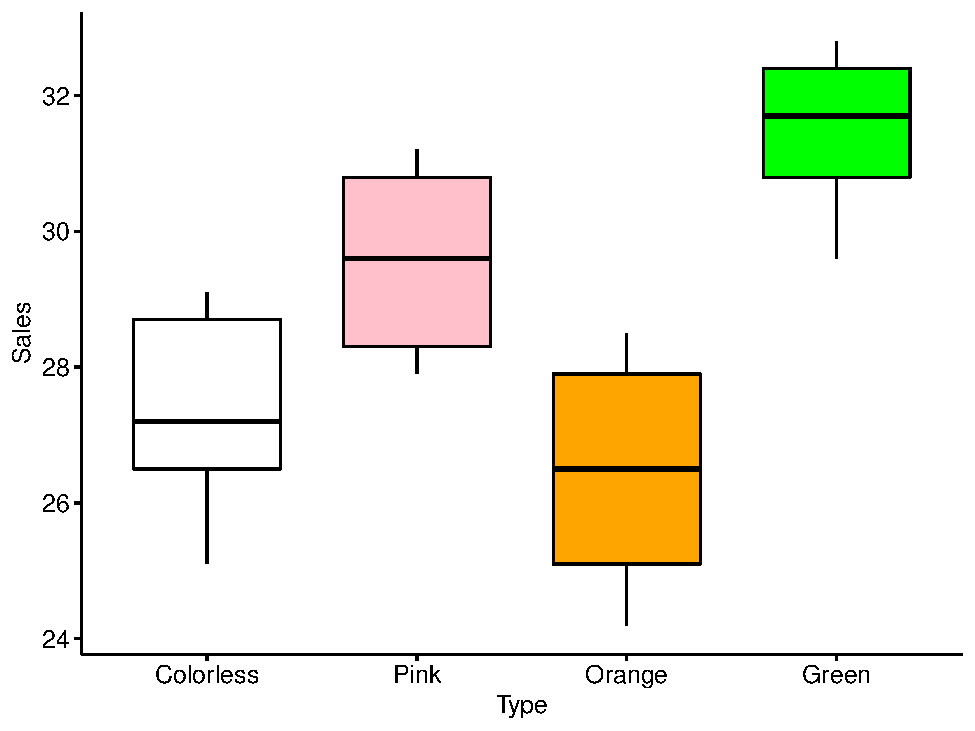
\includegraphics[width=0.8\linewidth]{_main_files/figure-latex/unnamed-chunk-8-1} \end{center}

\hypertarget{hypothesis-testing}{%
\chapter{Hypothesis Testing}\label{hypothesis-testing}}

\emph{The One-Way ANOVA Table in R}

\begin{Shaded}
\begin{Highlighting}[]
\NormalTok{one\_aov }\OtherTok{\textless{}{-}}\NormalTok{ clean\_oneway\_data }\SpecialCharTok{\%\textgreater{}\%} 
  \FunctionTok{aov}\NormalTok{(}\AttributeTok{formula =}\NormalTok{ Sales }\SpecialCharTok{\textasciitilde{}}\NormalTok{ Type, }\AttributeTok{data =}\NormalTok{ .)}
  
\NormalTok{one\_aov }\SpecialCharTok{\%\textgreater{}\%} 
\NormalTok{  summary}
\end{Highlighting}
\end{Shaded}

\begin{verbatim}
##             Df Sum Sq Mean Sq F value   Pr(>F)    
## Type         3  76.85  25.615   10.49 0.000466 ***
## Residuals   16  39.08   2.443                     
## ---
## Signif. codes:  0 '***' 0.001 '**' 0.01 '*' 0.05 '.' 0.1 ' ' 1
\end{verbatim}

In the table,

\begin{itemize}
\tightlist
\item
  \texttt{Df} -- degress of freedom
\item
  \texttt{Sum\ Sq} -- sum of squares
\item
  \texttt{Mean\ Sq} -- mean sum of squares
\item
  \texttt{F\ value} -- value of \(F\) statistic
\item
  \texttt{Pr(\textgreater{}F)} -- \(p\)-value
\end{itemize}

Thus, from the table

\begin{align}
    SSB &= 76.85 & MSB &= 25.615 & F = 10.49\\
    SSE &= 39.08 & MSE &= 2.443  & \\
  \end{align}

Similar to when you look up at an F-table, the p-value can be computed using the following R code.

\begin{Shaded}
\begin{Highlighting}[]
\FunctionTok{pf}\NormalTok{(}\AttributeTok{q =} \FloatTok{10.49}\NormalTok{, }\AttributeTok{df1 =} \DecValTok{3}\NormalTok{, }\AttributeTok{df2 =} \DecValTok{16}\NormalTok{, }\AttributeTok{lower.tail =}\NormalTok{ F)}
\end{Highlighting}
\end{Shaded}

\begin{verbatim}
## [1] 0.0004652698
\end{verbatim}

\hypertarget{checking-assumptions}{%
\chapter[Checking Assumptions]{\texorpdfstring{Checking Assumptions\footnote{Except for most of the codes, the contents of this section are obtained from this \href{https://yieldingresults.org/wp-content/uploads/2015/03/Checking_ANOVA_assumptions.html}{link}}}{Checking Assumptions}}\label{checking-assumptions}}

\hypertarget{checking-normality-assumptions}{%
\section{Checking Normality Assumptions}\label{checking-normality-assumptions}}

\emph{Shapiro-Wilk Test}

The Shapiro-Wilk test tests the null hypothesis that the samples come from a normal distribution against the alternative hypothesis that the samples do not come from a normal distribution.

\begin{Shaded}
\begin{Highlighting}[]
\NormalTok{oneway\_data[}\SpecialCharTok{{-}}\DecValTok{1}\NormalTok{,] }\SpecialCharTok{\%\textgreater{}\%} 
\NormalTok{  rstatix}\SpecialCharTok{::}\FunctionTok{shapiro\_test}\NormalTok{(Colorless,Pink,Orange,Green)}
\end{Highlighting}
\end{Shaded}

\begin{verbatim}
## # A tibble: 4 x 3
##   variable  statistic     p
##   <chr>         <dbl> <dbl>
## 1 Colorless     0.913 0.499
## 2 Green         0.881 0.342
## 3 Orange        0.965 0.813
## 4 Pink          0.937 0.635
\end{verbatim}

\begin{Shaded}
\begin{Highlighting}[]
\FunctionTok{shapiro.test}\NormalTok{(}\FunctionTok{residuals}\NormalTok{(}\AttributeTok{object =}\NormalTok{ one\_aov))}
\end{Highlighting}
\end{Shaded}

\begin{verbatim}
## 
##  Shapiro-Wilk normality test
## 
## data:  residuals(object = one_aov)
## W = 0.92472, p-value = 0.1222
\end{verbatim}

\emph{QQ Plots}

\begin{Shaded}
\begin{Highlighting}[]
\NormalTok{clean\_oneway\_data }\SpecialCharTok{\%\textgreater{}\%} 
  \FunctionTok{mutate}\NormalTok{(}\AttributeTok{Residual =}\NormalTok{ one\_aov}\SpecialCharTok{$}\NormalTok{residuals) }\SpecialCharTok{\%\textgreater{}\%} 
  \FunctionTok{ggplot}\NormalTok{(}\FunctionTok{aes}\NormalTok{(}\AttributeTok{sample =}\NormalTok{ Residual)) }\SpecialCharTok{+} 
  \FunctionTok{stat\_qq}\NormalTok{() }\SpecialCharTok{+} 
  \FunctionTok{stat\_qq\_line}\NormalTok{() }\SpecialCharTok{+} 
  \FunctionTok{facet\_wrap}\NormalTok{(}\SpecialCharTok{\textasciitilde{}}\NormalTok{Type)}
\end{Highlighting}
\end{Shaded}

\begin{center}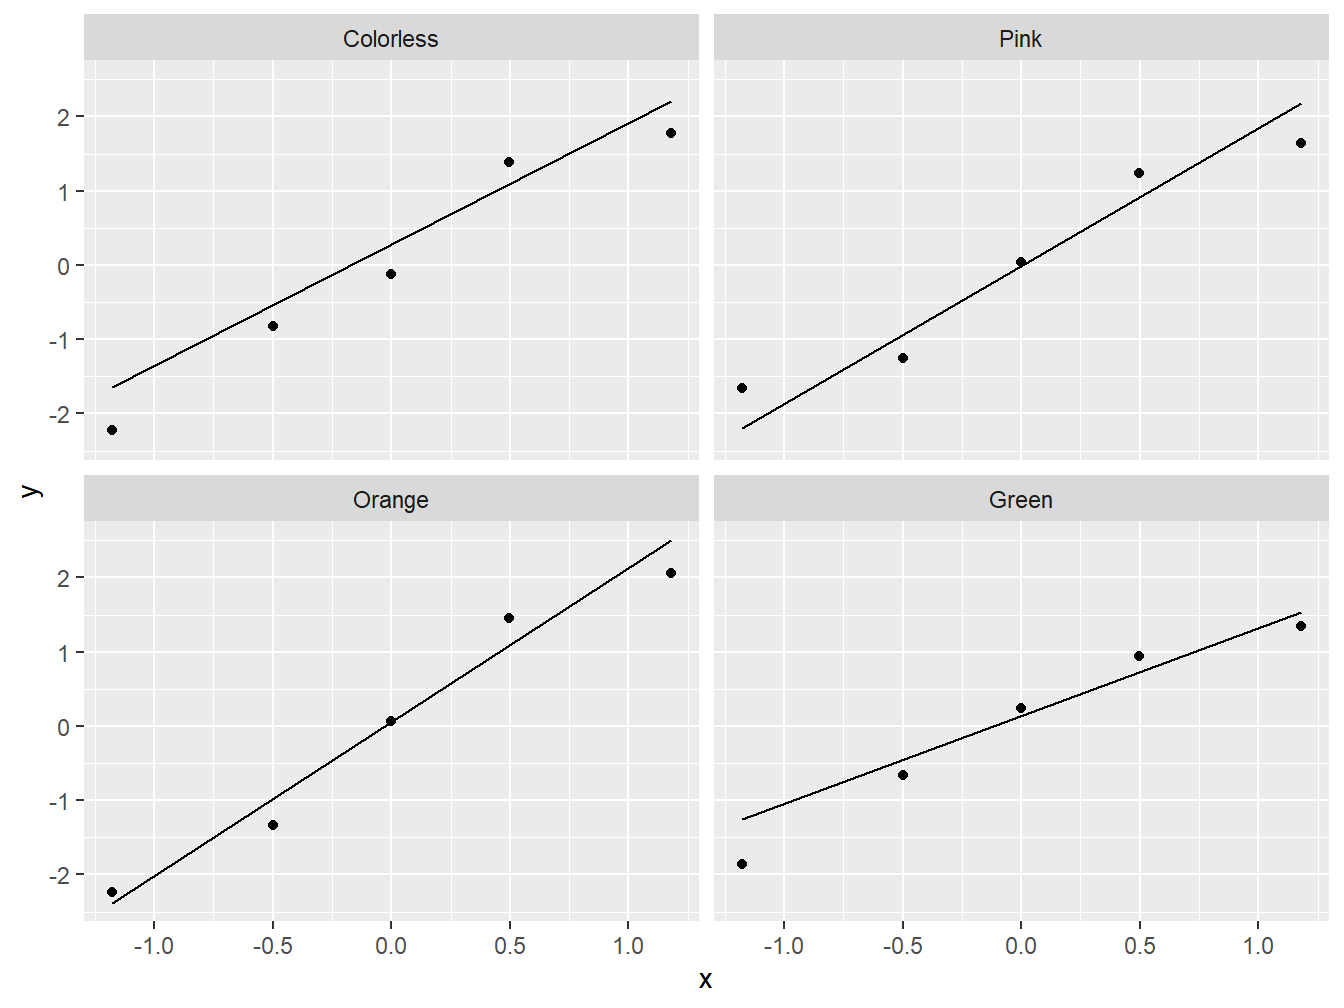
\includegraphics[width=0.8\linewidth]{_main_files/figure-latex/unnamed-chunk-13-1} \end{center}

\begin{Shaded}
\begin{Highlighting}[]
\FunctionTok{plot}\NormalTok{(one\_aov,}\DecValTok{2}\NormalTok{)}
\end{Highlighting}
\end{Shaded}

\begin{center}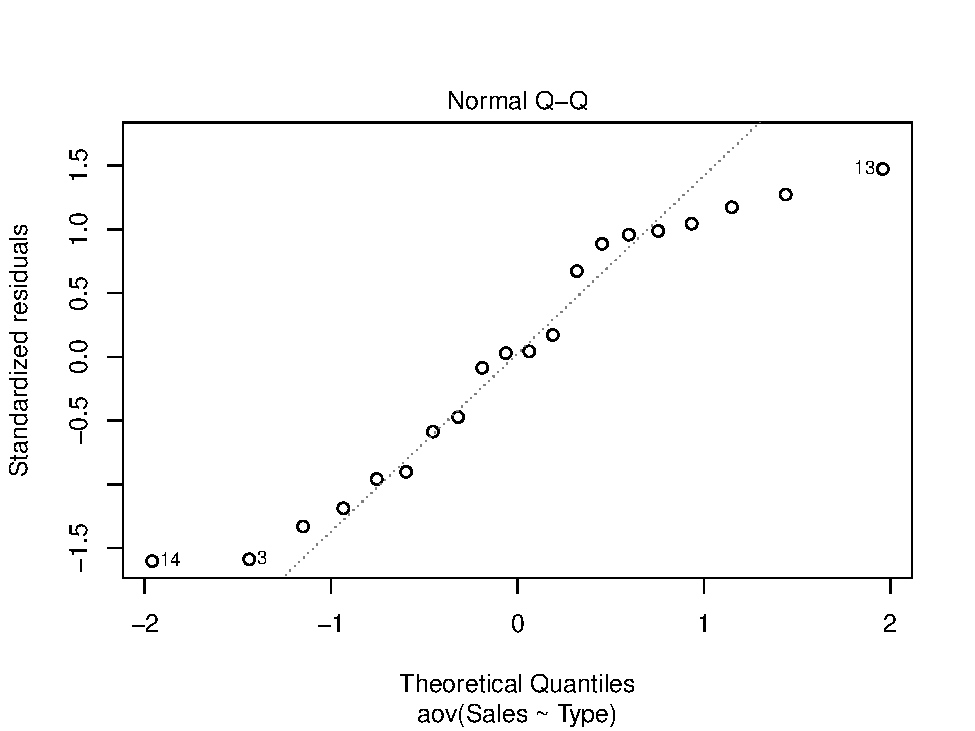
\includegraphics[width=0.8\linewidth]{_main_files/figure-latex/unnamed-chunk-14-1} \end{center}

\emph{Histogram}

\begin{Shaded}
\begin{Highlighting}[]
\NormalTok{clean\_oneway\_data }\SpecialCharTok{\%\textgreater{}\%} 
  \FunctionTok{ggplot}\NormalTok{(}\FunctionTok{aes}\NormalTok{(}\AttributeTok{x =}\NormalTok{ Sales)) }\SpecialCharTok{+} 
  \FunctionTok{geom\_histogram}\NormalTok{(}\AttributeTok{bins =} \DecValTok{30}\NormalTok{, }\AttributeTok{color =} \StringTok{"white"}\NormalTok{) }\SpecialCharTok{+} 
  \FunctionTok{geom\_density}\NormalTok{() }\SpecialCharTok{+} 
  \FunctionTok{facet\_wrap}\NormalTok{(}\SpecialCharTok{\textasciitilde{}}\NormalTok{Type)}
\end{Highlighting}
\end{Shaded}

\begin{center}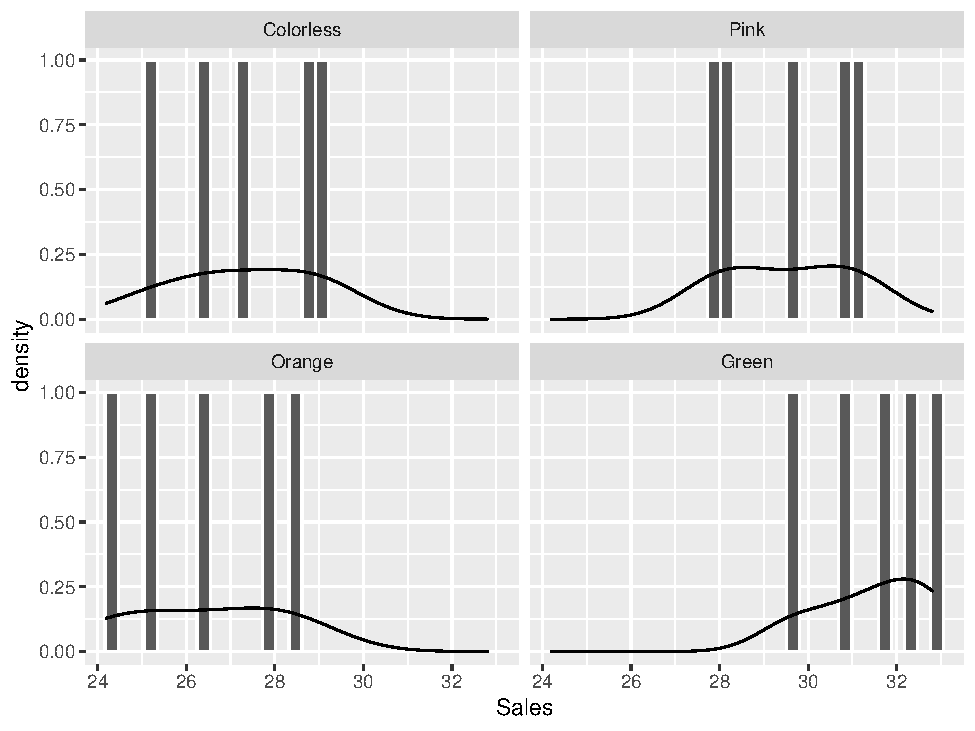
\includegraphics[width=0.8\linewidth]{_main_files/figure-latex/unnamed-chunk-15-1} \end{center}

\hypertarget{checking-homogeneity-of-variance-assumption}{%
\section{Checking Homogeneity of Variance Assumption}\label{checking-homogeneity-of-variance-assumption}}

\emph{Bartlet's Test}

Bartlett's test tests the null hypothesis that the group variances are equal against the alternative hypothesis that the group variances are not equal.

\begin{Shaded}
\begin{Highlighting}[]
\NormalTok{clean\_oneway\_data }\SpecialCharTok{\%\textgreater{}\%} 
  \FunctionTok{bartlett.test}\NormalTok{(Sales }\SpecialCharTok{\textasciitilde{}}\NormalTok{ Type, }\AttributeTok{data =}\NormalTok{ .)}
\end{Highlighting}
\end{Shaded}

\begin{verbatim}
## 
##  Bartlett test of homogeneity of variances
## 
## data:  Sales by Type
## Bartlett's K-squared = 0.46564, df = 3, p-value = 0.9264
\end{verbatim}

\begin{Shaded}
\begin{Highlighting}[]
\NormalTok{clean\_oneway\_data }\SpecialCharTok{\%\textgreater{}\%} 
  \FunctionTok{ggboxplot}\NormalTok{(}\AttributeTok{x =} \StringTok{"Type"}\NormalTok{, }\AttributeTok{y =} \StringTok{\textquotesingle{}Sales\textquotesingle{}}\NormalTok{,}
            \AttributeTok{fill =} \StringTok{"Type"}\NormalTok{,}
            \AttributeTok{palette =} \FunctionTok{c}\NormalTok{(}\StringTok{"white"}\NormalTok{, }\StringTok{"pink"}\NormalTok{, }\StringTok{"orange"}\NormalTok{, }\StringTok{"green"}\NormalTok{)) }\SpecialCharTok{+} 
  \FunctionTok{theme}\NormalTok{(}\AttributeTok{legend.position =} \StringTok{"none"}\NormalTok{)}
\end{Highlighting}
\end{Shaded}

\begin{center}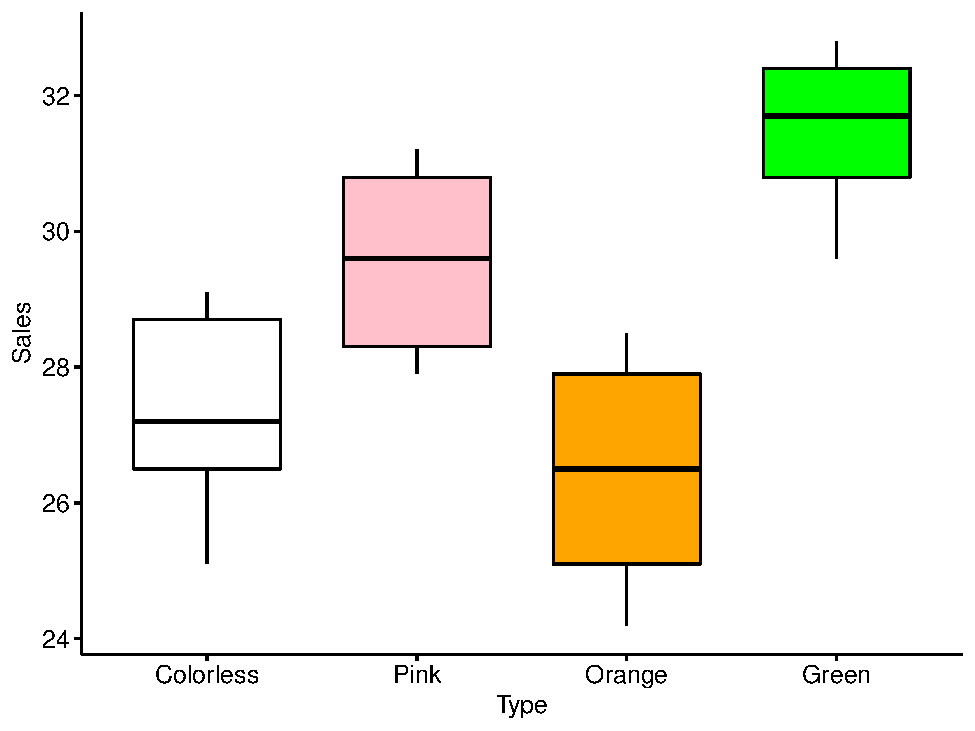
\includegraphics[width=0.8\linewidth]{_main_files/figure-latex/unnamed-chunk-17-1} \end{center}

The variability within each group is represented by the vertical size of each box; i.e., the interquartile range (IQR). The boxplot shows that the variability is roughly equal for each group. Let's look at some more ways to test the homogeneity of variance assumption.

\emph{Residual vs.~Fitted Values Plot}

\begin{Shaded}
\begin{Highlighting}[]
\FunctionTok{plot}\NormalTok{(one\_aov,}\DecValTok{1}\NormalTok{, }\AttributeTok{las=}\DecValTok{1}\NormalTok{)}
\end{Highlighting}
\end{Shaded}

\begin{center}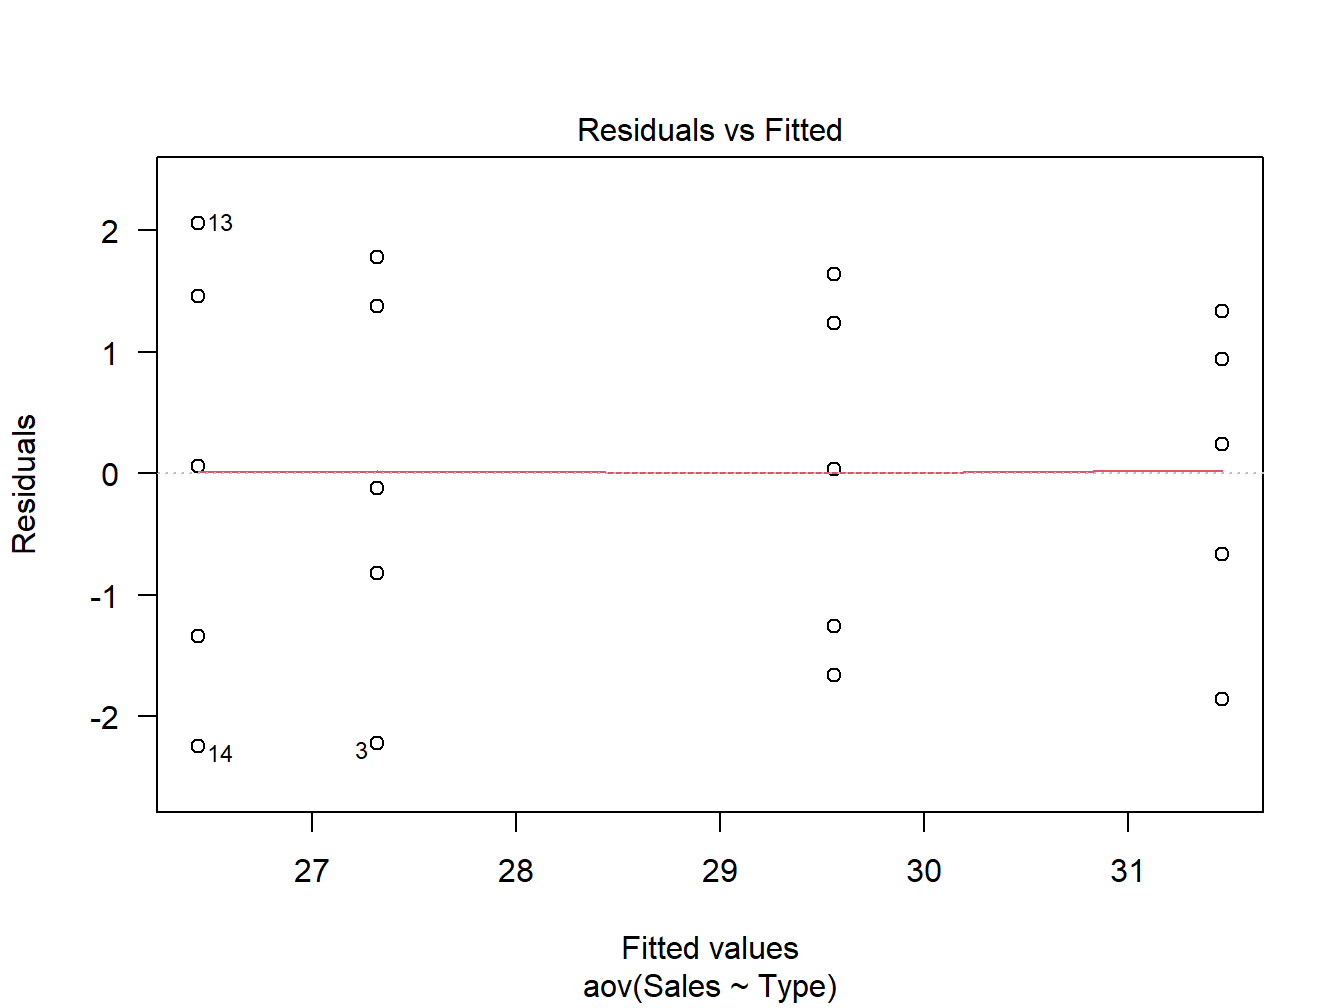
\includegraphics[width=0.8\linewidth]{_main_files/figure-latex/unnamed-chunk-18-1} \end{center}

This plot shows the residuals (errors) on the y-axis and the fitted values (predicted values) on the x-axis. If the variance of each group is equal, the plot should show no pattern; in other words, the points should look like a cloud of random points. The plot shows that the variances are approximately homogenous since the residuals are distributed approximately equally above and below zero.

\emph{Standardised Residuals vs Fitted values Plot}

\begin{Shaded}
\begin{Highlighting}[]
\FunctionTok{plot}\NormalTok{(one\_aov,}\DecValTok{3}\NormalTok{)}
\end{Highlighting}
\end{Shaded}

\begin{center}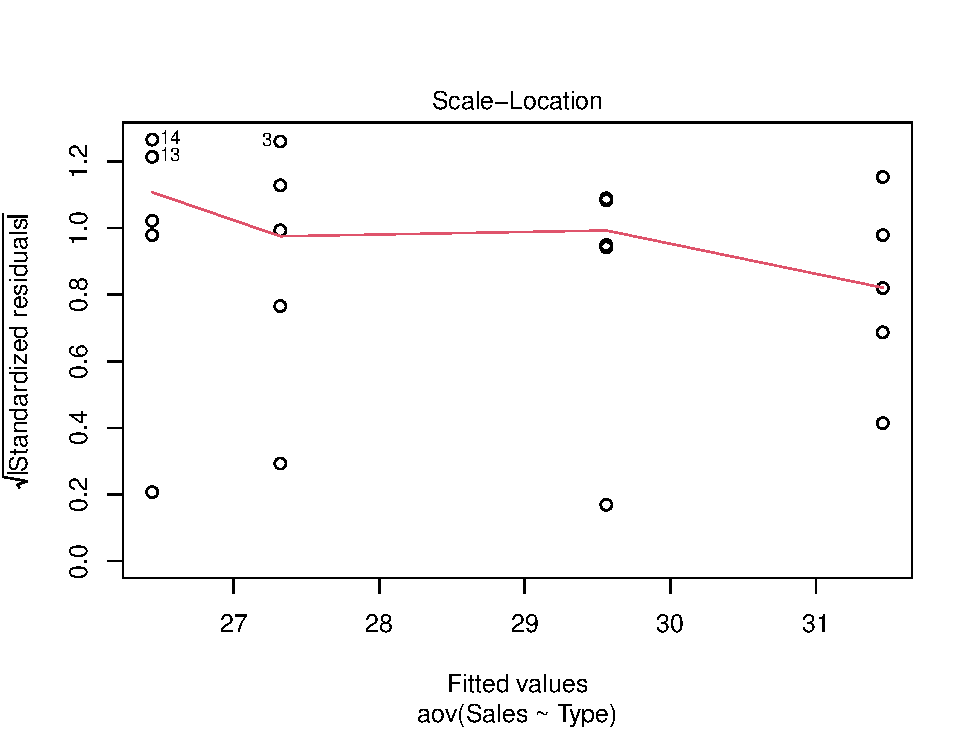
\includegraphics[width=0.8\linewidth]{_main_files/figure-latex/unnamed-chunk-19-1} \end{center}

The more coincident the red line plot to the horizontal line at 1, the lesser possibility the violation of the homogeneity of variance assumption.

\hypertarget{post-hoc}{%
\chapter{Post-hoc}\label{post-hoc}}

\hypertarget{tukeyhsd-tukeys-honestly-significant-difference-post-hoc-test-in-r}{%
\section{TukeyHSD (Tukey's Honestly-Significant Difference) post-hoc test in R}\label{tukeyhsd-tukeys-honestly-significant-difference-post-hoc-test-in-r}}

There are at least two ways to perform a Tukey's HSD post-hoc in R. One is by using the \texttt{TukeyHSD} function of the pre-installed R package \texttt{stats}. The second is the \texttt{glht} function with \texttt{"Tukey"} option bundled along with the \texttt{multcomp} package.

\hypertarget{using-tukeyhsd-of-stats-package}{%
\section{\texorpdfstring{Using \texttt{TukeyHSD} of \texttt{stats} package}{Using TukeyHSD of stats package}}\label{using-tukeyhsd-of-stats-package}}

\begin{Shaded}
\begin{Highlighting}[]
\FunctionTok{TukeyHSD}\NormalTok{(one\_aov)}
\end{Highlighting}
\end{Shaded}

\begin{verbatim}
##   Tukey multiple comparisons of means
##     95% family-wise confidence level
## 
## Fit: aov(formula = Sales ~ Type, data = .)
## 
## $Type
##                   diff        lwr        upr     p adj
## Pink-Colorless    2.24 -0.5880714  5.0680714 0.1479369
## Orange-Colorless -0.88 -3.7080714  1.9480714 0.8099459
## Green-Colorless   4.14  1.3119286  6.9680714 0.0034923
## Orange-Pink      -3.12 -5.9480714 -0.2919286 0.0281177
## Green-Pink        1.90 -0.9280714  4.7280714 0.2580535
## Green-Orange      5.02  2.1919286  7.8480714 0.0005837
\end{verbatim}

\textbf{\emph{Discussion of Results}}. Picking up from the significant ANOVA result in our soft drink data, the Tukey's HSD post-hoc analysis result above shows the following significant comparisons at \(0.05\):

\begin{Shaded}
\begin{Highlighting}[]
\FunctionTok{cat}\NormalTok{(}\StringTok{"Avg. Sales Comparison}\SpecialCharTok{\textbackslash{}t}\StringTok{ P{-}value (adjusted)}\SpecialCharTok{\textbackslash{}n}\StringTok{{-}{-}{-}{-}{-}{-}{-}{-}{-}{-}{-}{-}{-}{-}{-}{-}{-}{-}{-}{-}{-}{-}{-}{-}{-}{-}{-}{-}{-}{-}{-}{-}{-}{-}{-}{-}{-}{-}{-}{-}{-}{-}{-}{-}{-}}\SpecialCharTok{\textbackslash{}n}\StringTok{Green \textgreater{} Colorless}\SpecialCharTok{\textbackslash{}t}\StringTok{ 0.0034923}\SpecialCharTok{\textbackslash{}n}\StringTok{Green \textgreater{} Orange}\SpecialCharTok{\textbackslash{}t\textbackslash{}t}\StringTok{ 0.0005837}\SpecialCharTok{\textbackslash{}n}\StringTok{Orange \textgreater{} Pink}\SpecialCharTok{\textbackslash{}t\textbackslash{}t}\StringTok{ 0.0281177}\SpecialCharTok{\textbackslash{}n}\StringTok{{-}{-}{-}{-}{-}{-}{-}{-}{-}{-}{-}{-}{-}{-}{-}{-}{-}{-}{-}{-}{-}{-}{-}{-}{-}{-}{-}{-}{-}{-}{-}{-}{-}{-}{-}{-}{-}{-}{-}{-}{-}{-}{-}{-}{-}}\SpecialCharTok{\textbackslash{}n}\StringTok{"}\NormalTok{)}
\end{Highlighting}
\end{Shaded}

\begin{verbatim}
## Avg. Sales Comparison     P-value (adjusted)
## ---------------------------------------------
## Green > Colorless     0.0034923
## Green > Orange        0.0005837
## Orange > Pink         0.0281177
## ---------------------------------------------
\end{verbatim}

\hypertarget{using-the-multicomp-package-with-tukey-option}{%
\section{\texorpdfstring{Using the \texttt{multicomp} package with ``Tukey'' option}{Using the multicomp package with ``Tukey'' option}}\label{using-the-multicomp-package-with-tukey-option}}

\begin{Shaded}
\begin{Highlighting}[]
\FunctionTok{summary}\NormalTok{(}\FunctionTok{glht}\NormalTok{(one\_aov, }\AttributeTok{linfct =} \FunctionTok{mcp}\NormalTok{(}\AttributeTok{Type =} \StringTok{"Tukey"}\NormalTok{)))}
\end{Highlighting}
\end{Shaded}

\begin{verbatim}
## 
##   Simultaneous Tests for General Linear Hypotheses
## 
## Multiple Comparisons of Means: Tukey Contrasts
## 
## 
## Fit: aov(formula = Sales ~ Type, data = .)
## 
## Linear Hypotheses:
##                         Estimate Std. Error t value Pr(>|t|)    
## Pink - Colorless == 0     2.2400     0.9885   2.266  0.14815    
## Orange - Colorless == 0  -0.8800     0.9885  -0.890  0.80991    
## Green - Colorless == 0    4.1400     0.9885   4.188  0.00339 ** 
## Orange - Pink == 0       -3.1200     0.9885  -3.156  0.02817 *  
## Green - Pink == 0         1.9000     0.9885   1.922  0.25800    
## Green - Orange == 0       5.0200     0.9885   5.078  < 0.001 ***
## ---
## Signif. codes:  0 '***' 0.001 '**' 0.01 '*' 0.05 '.' 0.1 ' ' 1
## (Adjusted p values reported -- single-step method)
\end{verbatim}

\hypertarget{part-two-way-anova}{%
\part*{Two-Way ANOVA}\label{part-two-way-anova}}
\addcontentsline{toc}{part}{Two-Way ANOVA}

\hypertarget{data-entry-1}{%
\chapter[Data Entry]{\texorpdfstring{Data Entry\footnote{The contents of the succeeding sections are obtained from this \href{http://www.sthda.com/english/wiki/two-way-anova-test-in-r\#compute-two-way-anova-test-in-r-for-unbalanced-designs}{link}}}{Data Entry}}\label{data-entry-1}}

Load data to R using \texttt{read\_csv()} function of the \texttt{readr} package of \texttt{tidyverse} and save it with a variable name \texttt{twoway\_data}.

\begin{Shaded}
\begin{Highlighting}[]
\CommentTok{\# Load and save}
\NormalTok{twoway\_data }\OtherTok{\textless{}{-}} \FunctionTok{read\_csv}\NormalTok{(}\AttributeTok{file =} \StringTok{"data/Tubo{-}USEP\_Two{-}Way Cleaned Data for R.csv"}\NormalTok{)}
\CommentTok{\# Preview}
\NormalTok{twoway\_data}
\end{Highlighting}
\end{Shaded}

\begin{verbatim}
## # A tibble: 4 x 7
##   Fertilizer Manure    P1    P2    P3    P4    P5
##   <chr>      <chr>  <dbl> <dbl> <dbl> <dbl> <dbl>
## 1 High       High    13.7  15.8  13.9  16.6  15.5
## 2 High       Low     16.4  12.5  14.1  14.4  12.2
## 3 Low        High    15    15.1  12    15.7  12.2
## 4 Low        Low     12.4  10.6  13.7   8.7  10.9
\end{verbatim}

\hypertarget{data-manipulation-1}{%
\chapter{Data Manipulation}\label{data-manipulation-1}}

\begin{Shaded}
\begin{Highlighting}[]
\NormalTok{twoway\_data}\SpecialCharTok{\%\textgreater{}\%} 
  \FunctionTok{gather}\NormalTok{(}\AttributeTok{key =}\NormalTok{ Plot, }\AttributeTok{value =}\NormalTok{ Yield, }\SpecialCharTok{{-}}\FunctionTok{c}\NormalTok{(Fertilizer,Manure)) }\SpecialCharTok{\%\textgreater{}\%} 
  \FunctionTok{mutate}\NormalTok{(}\FunctionTok{across}\NormalTok{(Fertilizer}\SpecialCharTok{:}\NormalTok{Plot, }\SpecialCharTok{\textasciitilde{}} \FunctionTok{as.factor}\NormalTok{(.x))) }\OtherTok{{-}\textgreater{}}\NormalTok{ clean\_twoway\_data}
\end{Highlighting}
\end{Shaded}

\begin{Shaded}
\begin{Highlighting}[]
\CommentTok{\# Structure preview}
\FunctionTok{str}\NormalTok{(clean\_twoway\_data)}
\end{Highlighting}
\end{Shaded}

\begin{verbatim}
## tibble [20 x 4] (S3: tbl_df/tbl/data.frame)
##  $ Fertilizer: Factor w/ 2 levels "High","Low": 1 1 2 2 1 1 2 2 1 1 ...
##  $ Manure    : Factor w/ 2 levels "High","Low": 1 2 1 2 1 2 1 2 1 2 ...
##  $ Plot      : Factor w/ 5 levels "P1","P2","P3",..: 1 1 1 1 2 2 2 2 3 3 ...
##  $ Yield     : num [1:20] 13.7 16.4 15 12.4 15.8 12.5 15.1 10.6 13.9 14.1 ...
\end{verbatim}

\begin{Shaded}
\begin{Highlighting}[]
\CommentTok{\# Sample preview}
\NormalTok{clean\_twoway\_data }\SpecialCharTok{\%\textgreater{}\%} 
  \FunctionTok{sample\_n}\NormalTok{(}\DecValTok{10}\NormalTok{)}
\end{Highlighting}
\end{Shaded}

\begin{verbatim}
## # A tibble: 10 x 4
##    Fertilizer Manure Plot  Yield
##    <fct>      <fct>  <fct> <dbl>
##  1 High       High   P3     13.9
##  2 Low        Low    P5     10.9
##  3 High       High   P2     15.8
##  4 High       Low    P4     14.4
##  5 High       High   P5     15.5
##  6 High       Low    P2     12.5
##  7 Low        High   P3     12  
##  8 High       High   P1     13.7
##  9 High       Low    P3     14.1
## 10 Low        Low    P3     13.7
\end{verbatim}

\hypertarget{data-visualization-1}{%
\chapter{Data Visualization}\label{data-visualization-1}}

\begin{Shaded}
\begin{Highlighting}[]
\FunctionTok{ggboxplot}\NormalTok{(clean\_twoway\_data,}
          \AttributeTok{x =} \StringTok{"Fertilizer"}\NormalTok{,}
          \AttributeTok{y =} \StringTok{"Yield"}\NormalTok{,}
          \AttributeTok{fill =} \StringTok{"Manure"}\NormalTok{)}
\end{Highlighting}
\end{Shaded}

\begin{center}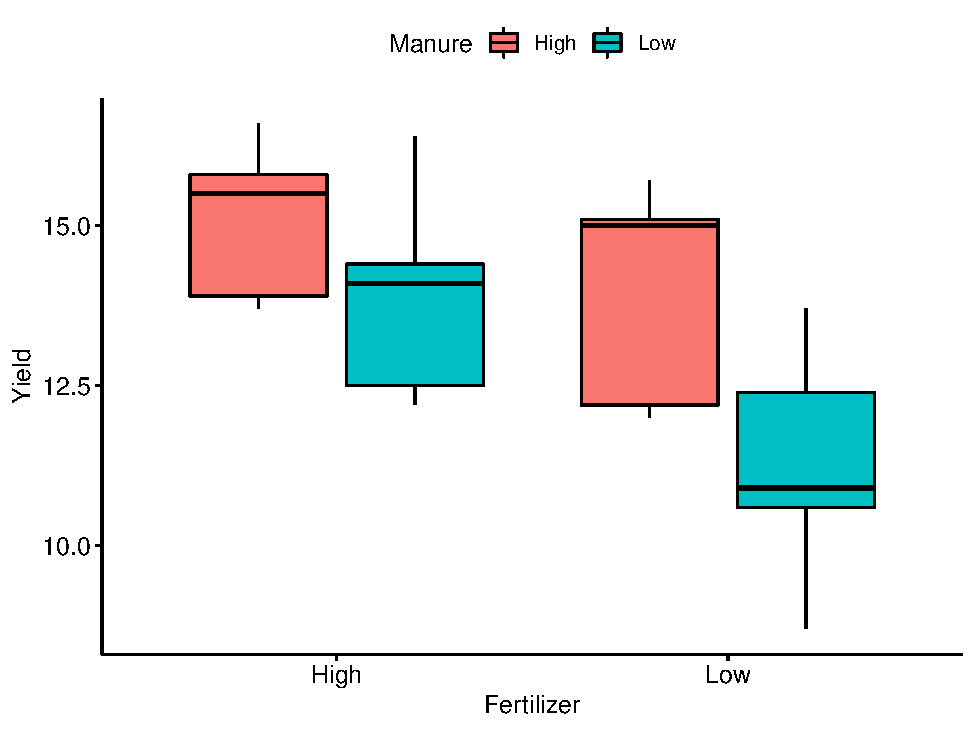
\includegraphics[width=0.8\linewidth]{_main_files/figure-latex/unnamed-chunk-27-1} \end{center}

\hypertarget{hypothesis-testing-1}{%
\chapter{Hypothesis Testing}\label{hypothesis-testing-1}}

\hypertarget{the-two-way-anova-table-with-main-effects-only}{%
\section{The Two-Way ANOVA Table with Main Effects Only}\label{the-two-way-anova-table-with-main-effects-only}}

\begin{Shaded}
\begin{Highlighting}[]
\NormalTok{two\_aov }\OtherTok{\textless{}{-}}\NormalTok{ clean\_twoway\_data }\SpecialCharTok{\%\textgreater{}\%} 
  \FunctionTok{aov}\NormalTok{(}\AttributeTok{formula =}\NormalTok{ Yield }\SpecialCharTok{\textasciitilde{}}\NormalTok{ Fertilizer }\SpecialCharTok{+}\NormalTok{ Manure, }\AttributeTok{data =}\NormalTok{ .)}
  
\NormalTok{two\_aov }\SpecialCharTok{\%\textgreater{}\%} 
\NormalTok{  summary}
\end{Highlighting}
\end{Shaded}

\begin{verbatim}
##             Df Sum Sq Mean Sq F value Pr(>F)  
## Fertilizer   1  17.67  17.672   6.332 0.0222 *
## Manure       1  19.21  19.208   6.883 0.0178 *
## Residuals   17  47.44   2.791                 
## ---
## Signif. codes:  0 '***' 0.001 '**' 0.01 '*' 0.05 '.' 0.1 ' ' 1
\end{verbatim}

Similar to the One-Way ANOVA table,

\begin{itemize}
\tightlist
\item
  \texttt{Df} -- degress of freedom
\item
  \texttt{Sum\ Sq} -- sum of squares
\item
  \texttt{Mean\ Sq} -- mean sum of squares
\item
  \texttt{F\ value} -- value of \(F\) statistic
\item
  \texttt{Pr(\textgreater{}F)} -- \(p\)-value
\end{itemize}

Thus, from the table

\begin{align}
    SSR &= 17.67 & MSR &= 17.672 & F_C = 6.332\\
    SSC &= 19.21 & MSC &= 19.208 & F_R = 6.883\\
    SSE &= 47.44 & MSE &= 2.791  & \\
  \end{align}

Similar to when you look up at an F-table, the p-values can be computed using the following R code.

\begin{Shaded}
\begin{Highlighting}[]
\FunctionTok{pf}\NormalTok{(}\AttributeTok{q =} \FloatTok{6.332}\NormalTok{, }\AttributeTok{df1 =} \DecValTok{1}\NormalTok{, }\AttributeTok{df2 =} \DecValTok{17}\NormalTok{, }\AttributeTok{lower.tail =}\NormalTok{ F)}
\end{Highlighting}
\end{Shaded}

\begin{verbatim}
## [1] 0.02219209
\end{verbatim}

\begin{Shaded}
\begin{Highlighting}[]
\FunctionTok{pf}\NormalTok{(}\AttributeTok{q =} \FloatTok{6.883}\NormalTok{, }\AttributeTok{df1 =} \DecValTok{1}\NormalTok{, }\AttributeTok{df2 =} \DecValTok{17}\NormalTok{, }\AttributeTok{lower.tail =}\NormalTok{ F)}
\end{Highlighting}
\end{Shaded}

\begin{verbatim}
## [1] 0.01779112
\end{verbatim}

\hypertarget{the-two-way-anova-table-with-interactions}{%
\section{The Two-Way ANOVA Table with Interactions}\label{the-two-way-anova-table-with-interactions}}

\begin{Shaded}
\begin{Highlighting}[]
\NormalTok{two\_aov2 }\OtherTok{\textless{}{-}}\NormalTok{ clean\_twoway\_data }\SpecialCharTok{\%\textgreater{}\%} 
  \FunctionTok{aov}\NormalTok{(}\AttributeTok{formula =}\NormalTok{ Yield }\SpecialCharTok{\textasciitilde{}}\NormalTok{ Fertilizer}\SpecialCharTok{*}\NormalTok{Manure, }\AttributeTok{data =}\NormalTok{ .)}
  
\NormalTok{two\_aov2 }\SpecialCharTok{\%\textgreater{}\%} 
\NormalTok{  summary}
\end{Highlighting}
\end{Shaded}

\begin{verbatim}
##                   Df Sum Sq Mean Sq F value Pr(>F)  
## Fertilizer         1  17.67  17.672   6.368 0.0226 *
## Manure             1  19.21  19.208   6.922 0.0182 *
## Fertilizer:Manure  1   3.04   3.042   1.096 0.3107  
## Residuals         16  44.40   2.775                 
## ---
## Signif. codes:  0 '***' 0.001 '**' 0.01 '*' 0.05 '.' 0.1 ' ' 1
\end{verbatim}

The interaction is not significant so we proceed on using the additive model (i.e., main-effects only).

\hypertarget{checking-assumptions-1}{%
\chapter{Checking Assumptions}\label{checking-assumptions-1}}

\hypertarget{checking-normality-assumptions-1}{%
\section{Checking Normality Assumptions}\label{checking-normality-assumptions-1}}

\emph{Shapiro-Wilk Test}

The Shapiro-Wilk test tests the null hypothesis that the samples come from a normal distribution against the alternative hypothesis that the samples do not come from a normal distribution.

\begin{Shaded}
\begin{Highlighting}[]
\FunctionTok{shapiro.test}\NormalTok{(}\FunctionTok{residuals}\NormalTok{(two\_aov))}
\end{Highlighting}
\end{Shaded}

\begin{verbatim}
## 
##  Shapiro-Wilk normality test
## 
## data:  residuals(two_aov)
## W = 0.9634, p-value = 0.6138
\end{verbatim}

\emph{QQ Plots}

\begin{Shaded}
\begin{Highlighting}[]
\FunctionTok{plot}\NormalTok{(two\_aov, }\DecValTok{2}\NormalTok{)}
\end{Highlighting}
\end{Shaded}

\begin{center}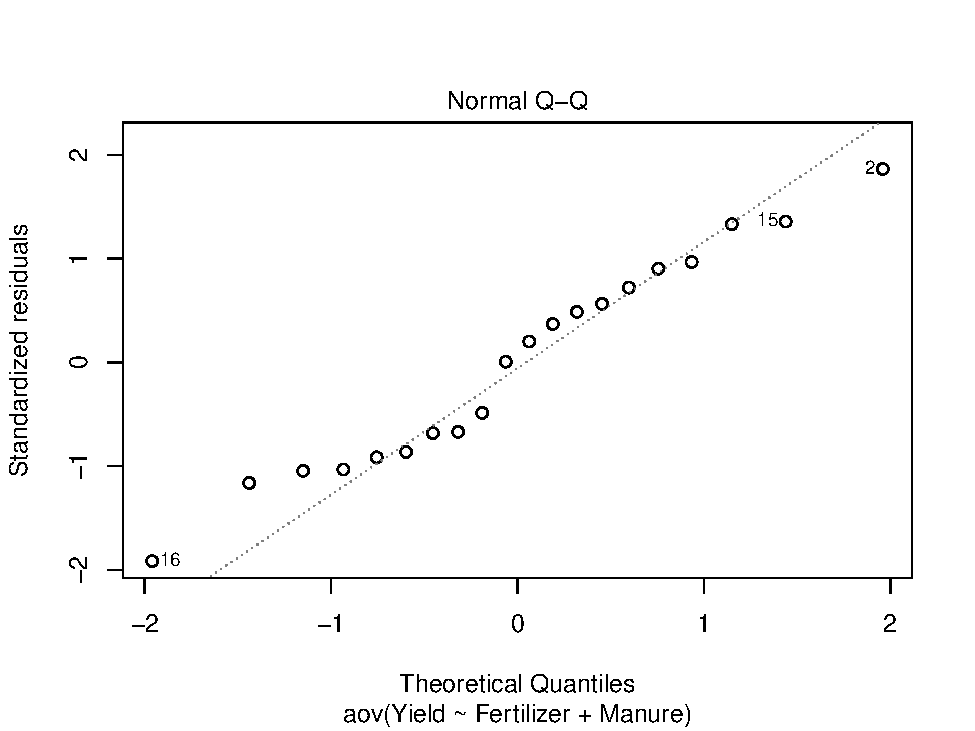
\includegraphics[width=0.8\linewidth]{_main_files/figure-latex/unnamed-chunk-32-1} \end{center}

\hypertarget{checking-homogeneity-of-variance-assumption-1}{%
\section{Checking Homogeneity of Variance Assumption}\label{checking-homogeneity-of-variance-assumption-1}}

\begin{Shaded}
\begin{Highlighting}[]
\FunctionTok{par}\NormalTok{(}\AttributeTok{mfrow=}\FunctionTok{c}\NormalTok{(}\DecValTok{2}\NormalTok{,}\DecValTok{2}\NormalTok{))}
\FunctionTok{plot}\NormalTok{(two\_aov)}
\end{Highlighting}
\end{Shaded}

\begin{center}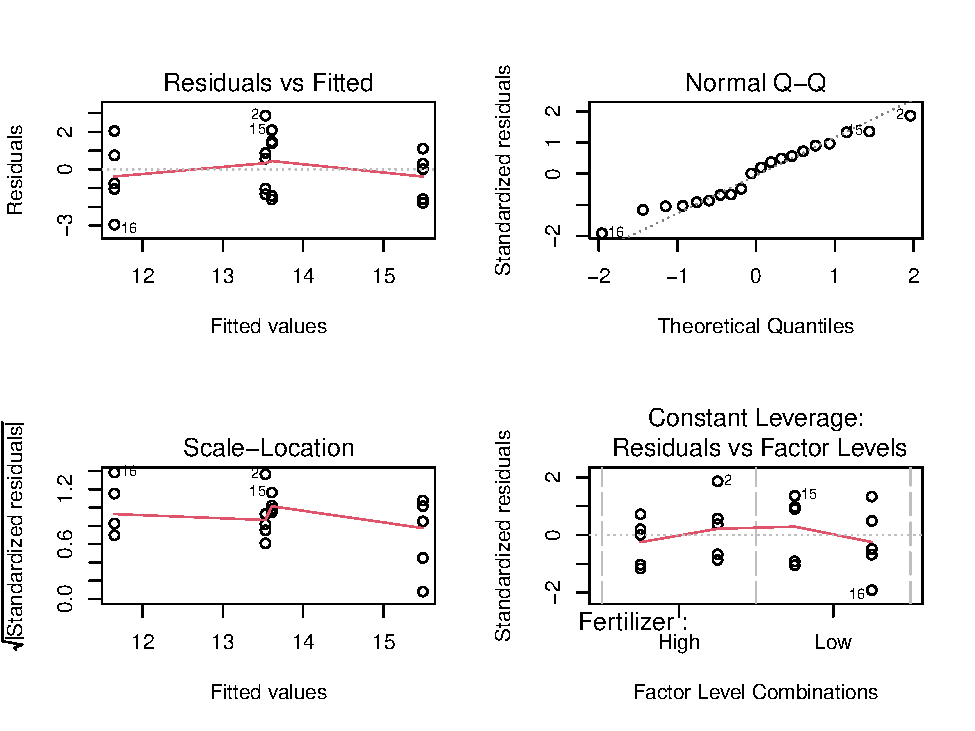
\includegraphics[width=0.8\linewidth]{_main_files/figure-latex/unnamed-chunk-33-1} \end{center}

\begin{Shaded}
\begin{Highlighting}[]
\FunctionTok{par}\NormalTok{(}\AttributeTok{mfrow=}\FunctionTok{c}\NormalTok{(}\DecValTok{1}\NormalTok{,}\DecValTok{1}\NormalTok{))}
\end{Highlighting}
\end{Shaded}

\hypertarget{post-hoc-1}{%
\chapter{Post-hoc}\label{post-hoc-1}}

We no longer need a posthoc analysis since we only have two levels in each of the significant factors. However, for the sake of illustration, we could be simply run the following code

\begin{Shaded}
\begin{Highlighting}[]
\FunctionTok{TukeyHSD}\NormalTok{(two\_aov)}
\end{Highlighting}
\end{Shaded}

\begin{verbatim}
##   Tukey multiple comparisons of means
##     95% family-wise confidence level
## 
## Fit: aov(formula = Yield ~ Fertilizer + Manure, data = .)
## 
## $Fertilizer
##           diff       lwr        upr    p adj
## Low-High -1.88 -3.456219 -0.3037812 0.022188
## 
## $Manure
##           diff       lwr        upr     p adj
## Low-High -1.96 -3.536219 -0.3837812 0.0177922
\end{verbatim}

\hypertarget{mean-line-or-interaction-plots}{%
\chapter{Mean Line or Interaction Plots}\label{mean-line-or-interaction-plots}}

\begin{Shaded}
\begin{Highlighting}[]
\FunctionTok{ggline}\NormalTok{(clean\_twoway\_data,}
       \AttributeTok{x =} \StringTok{"Fertilizer"}\NormalTok{,}
       \AttributeTok{y =} \StringTok{"Yield"}\NormalTok{,}
       \AttributeTok{color =} \StringTok{"Manure"}\NormalTok{,}
       \AttributeTok{add =} \FunctionTok{c}\NormalTok{(}\StringTok{"mean\_se"}\NormalTok{))}
\end{Highlighting}
\end{Shaded}

\begin{center}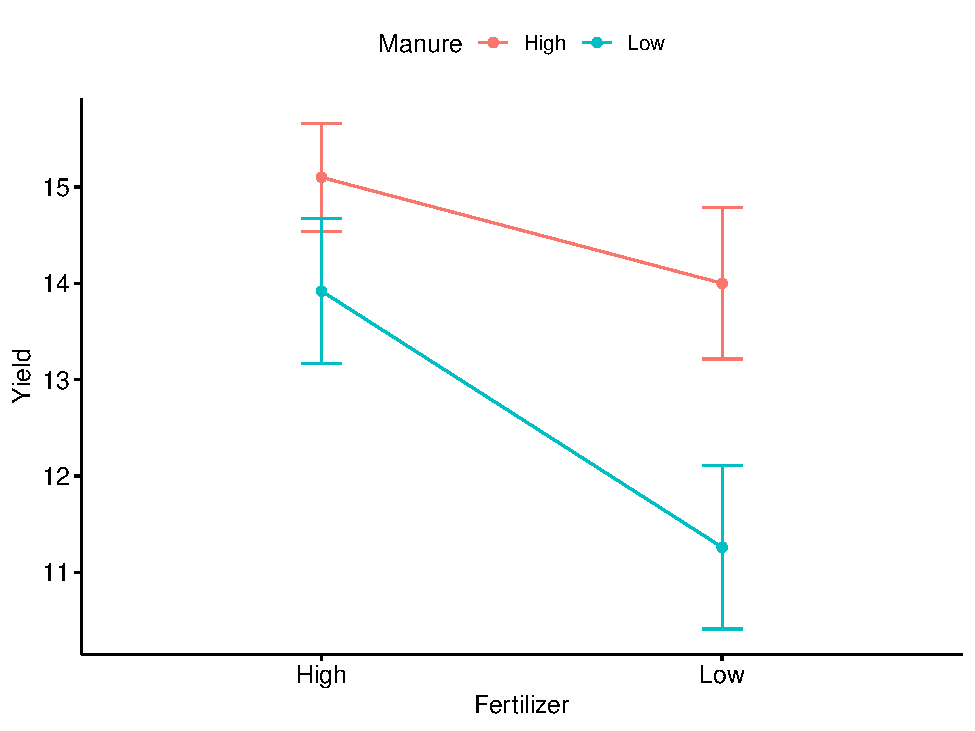
\includegraphics[width=0.8\linewidth]{_main_files/figure-latex/unnamed-chunk-35-1} \end{center}

The above figure supports the result before that there is no significant interaction between the two factors.

  \bibliography{book.bib,packages.bib}

\end{document}
